\section{Base de datos de artículos}
La instancia seleccionada para realizar las pruebas de lo propuesto en este trabajo es sobre la base de datos de los artículos de \textit{\textquotedblleft A Data-Driven Journey through Software Engineering Research\textquotedblright}\cite{dataDrive}. La decisión de utilizar esta base de datos es por la completitud de la información y que la cantidad de elementos que contiene requiere de algoritmos eficientes. La base de datos contiene cerca de $7800$ artículos, de los que se tiene los autores, de la conferencia en que fueron presentados y clasificados en tópicos. Ésta clasificación es llamada \texttt{topicProfile} y esta expresada en porcentajes para cada uno de tópicos que son tratados. De los $9800$ autores se tiene la información de que a universidad pertenecen y además de cada una de las universidades se sabe a que región pertenece cada una.\\
El \texttt{topicProfile} es lo que permitirá definir la similitud no sólo entre los artículos, sino que también entre los autores y las universidades de la base da datos de una manera prácticamente directa.\\

Para las pruebas, los criterios de las búsquedas que se realizaron sobre la base de datos se concibieron a partir de lo que se consideró que tiene un interés general. Por ejemplo, quiénes son los autores que escribieron artículos similares de distintas universidades o las universidades de diferentes regiones donde se escribieron artículo de los mismos tópicos.\\
Por lo establecido en \cite{compositeRetrival} para las búsquedas se deben realizar las siguientes definiciones:
\begin{itemize}
  \item \textbf{Similitud}: Función que dado dos ítems devuelve la similitud entre estos.
  \item \textbf{Costo}: Función que dado un ítem devuelve el costo del mismo.
  \item \textbf{Presupuesto}: El presupuesto que se tiene, el cual no podrá ser excedido por ningún bundle.
  \item \textbf{Complmentariedad}: Propiedad del ítem que es único en cada bundle.
\end{itemize}
Para todas las búsquedas, sin importar el ítem que sea (artículo, autores o universidades),  se definió que el costo de cada ítem sea de una unidad y que el presupuesto para cada búsqueda es de cinco unidades. Por lo que en todos los resultados se obtienen bundles que contienen como máximo cinco ítems; además se deicidió que sean diez los bundles devueltos en cada búsqueda. El motivo es para que sea fácil para un humano valorizar el resultado propuesto. Entonces de aquí en adelante para cada criterio de búsqueda se deben definir únicamente la función de similitud y la propiedad de complementariedad.\\
Como se mencionó anteriormente, en la base de datos cada artículo cuenta con su \texttt{Topic Profile}. El \texttt{Topic Profile} define el perfil de cada artículo asignándole un porcentaje a cada tópico que se hace referencia. En el caso del artículo \texttt{A Cognitive-Based Mechanism for Constructing Software Inspection Teams} el \texttt{Topic Profile} se compone por los tópicos  REQUIREMENTS, RELIABILITY, TESTING y SOFTWARE QUALITY el porcentaje de cada uno de estos es 71.43 \%, 17.86 \%, 7.14 \% y 3.57 \% respectivamente. \\
De los autores no se cuenta con una información directa que defina el perfil, entonces el perfil de los autores se genera a partir de los artículos que escribieron. Para definir el perfil de las universidades se aplicó el perfil de los autores definidos anteriormente. Más adelante se verá como se utilizan los perfiles para definir la función de similitud entre los ítems. A continuación se detallan las consultas realizadas en este trabajo.\\
Se utilizaron los siguientes criterios a las consultas que se hicieron en la base de datos, en los cuales la función costo para todos los elementos se defino con la constante 1 y el presupuesto de 5. Se decidió así porque no tiene sentido asociarle un costo a los artículos, autores, universidades y solo nos interesa que el bundle tengo como máximo un número fijo de elementos. Entonces de aquí en adelante para cada criterio solo resta definir la función de similitud y la propiedad de complementariedad.

\subsection{Artículos de diferentes conferencias}\label{bus:papSimDisLug}
Generar una solución, en el que cada bundle contenga artículos similares que se hayan presentado en distintas conferencias.\\
\begin{itemize}
  \item \textbf{Similitud}: Función que compara el perfil de cada artículo.
  \item \textbf{Complementariedad}: Lugar dónde fue presentado.
\end{itemize}

\subsection{Autores de distintas universidades}
Solución de bundles en el que cada uno contiene autores similares de distinta universidad de afiliación.\\
\begin{itemize}
  \item \textbf{Similitud}: Función que compara el perfil de los autores.
  \item \textbf{Complementariedad}: Universidad de pertenencia del autor.
\end{itemize}

\subsection{Instituciones de diferentes regiones}
En este caso, la búsqueda es para instituciones de diferentes regiones. 
\begin{itemize}
  \item \textbf{Similitud}: Función que compara el perfil de las instituciones.
  \item \textbf{Complementariedad}: Región de la institución.
\end{itemize}

Como se menciona antes, la base de datos cuenta con un \texttt{Topic Profile} de cada artículo que es un porcentaje del tema al que hace referencia. Esto se puede transformar a un vector de $n$ dimensiones en dónde cada posición representa un tópico diferente, entonces para cada artículo se obtiene un vector de la misma dimensión. Ésto es clave para la generación de la similitud entre los artículos.\\
Para los autores no se cuenta con información más allá de los artículos que escribieron, pero sólo con eso alcanza para poder generar un perfil de autores, por lo tanto para cada autor se hace la suma vectorial de cada uno de los \texttt{Topic Profile} de los artículos en los cuales participó y con eso se obtiene el \texttt{Topic Profile de Autores}.Para obtener el perfil de las universidades se aplicó el mismo criterio que para los autores, de hacer la suma vectorial de cada uno de los \texttt{Topic Profile de Autores} pertenecientes a la misma universidad y así generar el \texttt{Topic Profile de Universidades}. En ambos casos se aplica la normalización sobre los vectores resultantes.

Ejemplo de los perfiles de los elementos:

\begin{description}
 \item[Artículo - Topic Profile - Autores]
 \item Artículo 1 - $[$0.20, 0.40, 0.40, 0.00$]$ - Autor 1, Autor 2, Autor 3
 \item Artículo 2 - $[$0.30, 0.70, 0.00, 0.00$]$ - Autor 2, Autor 3
 \item Artículo 3 - $[$0.00, 0.10, 0.00, 0.90$]$ - Autor 2
 \item Artículo 4 - $[$0.00, 0.00, 1.00, 0.00$]$ - Autor 1, Autor 3
\end{description}

\begin{description}
 \item[Autor - Topic Profile - Universidad]
 \item Autor 1 - $[$0.14, 0.27, 0.95, 0.00$]$ - Universidad 1
 \item Autor 2 - $[$0.30, 0.74, 0.25, 0.55$]$ - Universidad 2
 \item Autor 3 - $[$0.27, 0.60, 0.76, 0.0$]$ - Universidad 2
\end{description}

\begin{description}
 \item[Universidad - Topic Profile]
 \item Universidad 1 - $[$0.14, 0.27, 0.95, 0.00$]$
 \item Universidad 2 - $[$0.31, 0.72, 0.54, 0.30$]$
\end{description}

\subsection{Función de similitud}
La similitud se emplea para comparar dos objetos y determinar qué tan parecido son entre si. En este trabajo para determinar la similitud entre los objetos es por la medida conocida como \textbf{similitud coseno}. Esta es una medida de similitud entre dos vectores en un espacio vectorial provisto de un producto escalar que mide el coseno del ángulo comprendido entre ellos. El coseno para el ángulo cero es 1, es menor a 1 para cualquier otro ángulo y es 0 cuando los vectores son ortogonales. De esta forma lo que define la similitud de los vectores es la orientación y no así la magnitud.\\
Entonces se define la función de similitud $S(V_i, V_j)$ para los vectores $V_i$ y $V_j$ a partir del producto escalar\\

\begin{equation} \label{eq:angulovectorial}
\cos(\theta) =  \dfrac{\overrightarrow{U} . \overrightarrow{V}}{\overrightarrow{\lVert V\lVert}.\overrightarrow{\lVert U\lVert}}
\end{equation}

Para esta instancia los objetos (ahora artículos, autores o universidades) son representados por vectores, donde cada dimensión corresponde a un tópico y el valor se corresponde con el valor del tópico del objeto según la base de datos \cite{dataDrive}. Por lo tanto el objeto $a$ se representa con el vector $V_a = [v_1,v_2,...,v_n]$, donde $N$ es la cantidad de tópicos y cumple con las siguientes propiedades:
\begin{enumerate}
 \item $v_i \geq 0$
 \item $\sum{v_i} = 1$
\end{enumerate}

Como los componentes de todos los vectores son mayor o igual a cero se obtiene que $0\leq\cos(\theta)\leq1$, que implica que $S(V_i, V_j) \in \left[0, 1\right]$.\\

\begin{figure}[H]
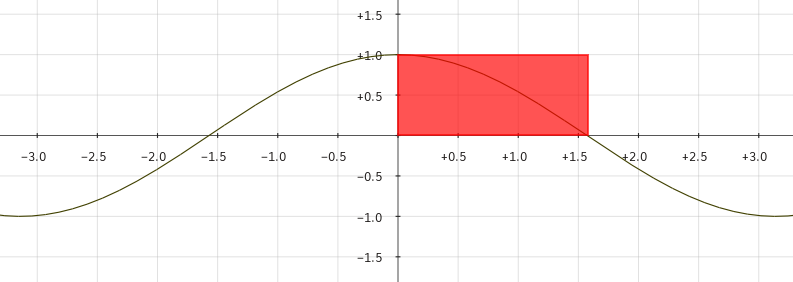
\includegraphics[width=0.8\textwidth]{img/coseno.png}
\caption{Comportamiento de la función $\cos$. En rojo la región que pertenece a la función de similitud}
\label{bus:img-coseno}
\end{figure}

Dos vectores proporcionales tiene la misma dirección y el ángulo entre ellos es cero, entonces la función de similitud es 1. Lo que significa que esta medida de similitud no considera el peso de cada tópico, por lo tanto no diferencia entre un artículo profesional y un artículo de un diario que cubre el mismo tópico. Esta debilidad de la medida basada en el ángulo no interfiere en este trabajo por la segunda propiedad de los vectores del problema, porque para que dos vectores sean proporcionalmente iguales tienen que ser idénticos y en tal caso es correcto que la similitud entre ellos sea 1.
\section{Atracciones turísticas}
Se dispuso de una instancia de datos correspondiente a 200 atracciones turísticas de Europa que contienen la información del valor de la visita, que tipo de visita es (parque, musea, edificio) y cual es la similitud entre ellas. Las búsquedas que se hicieron para este problema tienen como objetivo obtener grupos de lugares turísticos que pueden ser visitados por un viajante en el que cada grupo los elementos pertenecen a un tipo de visita diferente y el valor total de sus costos no excede el presupuesto asignado.\\
